\documentclass[tikz,border=2pt]{standalone}
\pdfmapfile{+cm.map}
\usepackage{pgfplots}
\pgfplotsset{compat=1.18}
\usetikzlibrary{arrows.meta}
\definecolor{ink}{HTML}{202B30}
\definecolor{red}{HTML}{971D2C}
\definecolor{soft}{HTML}{F4E9EB}
\definecolor{gray}{HTML}{51636D}
\definecolor{line}{HTML}{D6DDE0}
\definecolor{pale}{HTML}{F0F3F4}
\begin{document}
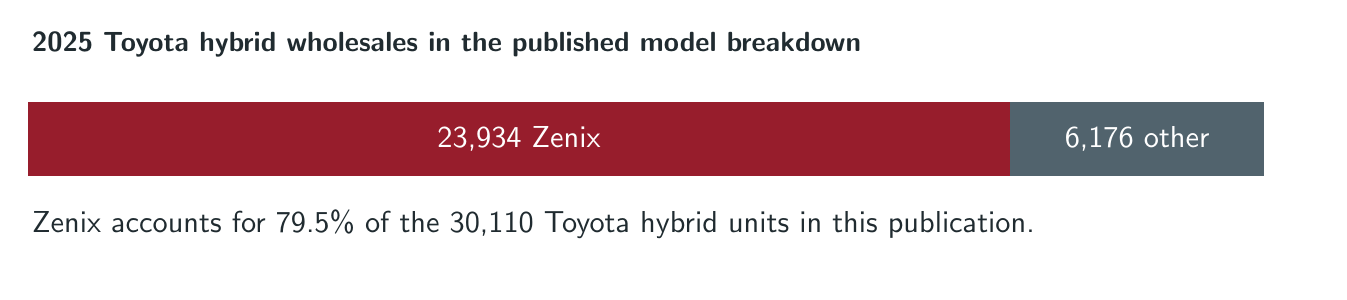
\begin{tikzpicture}[x=1cm,y=1cm,font=\sffamily\fontsize{10.5}{12}\selectfont,text=ink,arr/.style={-{Stealth[length=2mm]},draw=gray,thick}]
\path[use as bounding box] (0,0) rectangle (16.4,3.1);
\node[anchor=west,inner sep=0pt,font=\sffamily\bfseries] at (0.05,2.88) {2025 Toyota hybrid wholesales in the published model breakdown};
\fill[red] (0,1.22) rectangle (12.48,2.16);
\node[align=center,inner sep=0pt,text=white] at (6.24,1.69) {23,934 Zenix};
\fill[gray] (12.48,1.22) rectangle (15.700000000000001,2.16);
\node[align=center,inner sep=0pt,text=white] at (14.09,1.69) {6,176 other};
\node[anchor=west,inner sep=0pt,] at (0.05,0.61) {Zenix accounts for 79.5\% of the 30,110 Toyota hybrid units in this publication.};
\end{tikzpicture}\end{document}